\documentclass[12pt]{article}
\usepackage{amsmath}
\usepackage{graphicx}
\begin{document}
We used a cylindrical cavity cooled to $\sim 5$ K resonant at a frequency of $33.9-34.5$ GHz in the $\text{�}_{020}$ mode. The cavity was tuned to a specific resonant frequency using a dielectric rod; we measured the resonant frequency and Q using a vector network analyzer, then recorded the amplified noise from the cavity (after being mixed down to baseband) for an hour before retuning the cavity by 3 MHz. The baseband noise when Fourier transformed is a measure of the power in each frequency interval $\delta f$ that is the sum of the power in the cavity plus additional noise from the receiver chain. 

We recorded data in twelve separate runs (Nov 19 to May 30, 2014), and measured noise for 500 settings of the cavity frequency, with an hour of integration. The actual performance of our system

Summary of Runs
\begin{center}
\begin{tabular}{c | c | c }\hline
\hline
Run & No. of Freq.'s & State \\ \hline \hline
11/19-11/22 & 9 & slow DAQ \\ \hline
12/03-12/07 & 39 & faster DAQ \\ \hline
12/10-12/13 & 22 & tuning rod froze\\ \hline
12/16-12/20 & 27 & --\\ \hline
01/08-01/11 & 46 & heater feedback loop online\\ \hline
01/14-01/18 & 69 & RF switch added \\ \hline
01/23 & 5 & -- \\ \hline
01/28-02/01 & 41 & test tone added \\ \hline
02/04-02/07 & 33 & tuning rod froze\\ \hline
02/11-02/13 & 19 & -- \\ \hline
03/10-03/13 & 16 & -- \\ \hline
05/06-05/09 & x & weak coupling port altered, test tone removed\\ \hline
05/14-05/17 & x & -- \\ \hline
05/28-05/30 & x & -- \\ \hline
\hline
\end{tabular}
\label{table:runsummary}
\end{center}
\section{Procedure}

We tracked the in-phase and quadrature voltage of our baseband signal for an hour at each frequency setting. To allow for overlap between the covered frequencies, the cavity resonance was shifted by 3 MHz at a time. The dominant systematic effects were temperature variations in the cryostat. 

To reduce the effects of the the temperature shifts we discarded all data that was greater than 28 sigma away from the first minute of data. 

The data presented here were taken during 2014 Nov 19-22, Dec 05 to 07, 11 to 13, � . These runs gave a total of 500 hours of useful data. After correcting the data for the gain of the receiver and converting them to thermodynamic temperatures we compute the mean values $\Delta T_{bin}^i$ for the observations of each frequency bin of width $\delta f$ for each spectrum. The corresponding standard deviations, $\sigma_{bin}^i$ are calculated from the scatter of the individual 57 second measurements and are an estimate of the statistical uncertainty in the mean of an hour of data. ADDINBOOTSTRAP A typical value for data taken at 5 K is $\sigma_{bin189}^i = 0.25 mK$ whereas one expects $0.14$ mK from system noise alone. The excess noise at this stage is due to the $1/f$ component and in the variable temperature noise.

The final values $\bar \Delta T_{bin}^i$ for each one of the bins were obtained by weighting by $(\sigma_{bin}^i)^2$ each one of the hour observations for a given bin. The results are plotted in Figure 1 and show no statistically significant signal in any of the bins. The errors associated to each point correspond to the standard deviations estimated from the measurement statistics in the usual way. As the data will be used to decide what level of axion coupling is excluded by these measurements it is crucial to estimate the errors in Figure 1 accurately. The scatter in the values of $\Delta T_f^i$ for the different measurements could be larger than expected from the systematic effects. In principle, one could perform standard Chi-square tests for each one of the bins. Any such test would compare the scatter of the different observations of a given field with respect to the final value, with the corresponding values of $\sigma$. Let me emphasize that such a test does not depend on whether there is a true signal coming from the sky, as the scatter is computed with respect tone "local mean"; it is truly an instrumental Chi-square test. Figure 2 shows a histogram of the weighted residuals $(\Delta T - \bar \Delta T)\sigma$ for the observations. The histogram is reasonably gaussian with the a width that is consistent with what we would expect if all the scatter the values of $\Delta T$ with respect to their corresponding average value were due to fluctuations contained in $\sigma_i$. Indeed, the corresponding value of Chi-Square is of 78 with 75 degrees of freedom. Therefore, we conclude that it is legitimate to estimate the standard deviations $\bar \sigma$ in the standard way, as $\bar \sigma = [\Sigma \sigma^{-2}]^{-1/2}$. The variation of $\sigma$ frm bin to bin is mainly due to the different number of runs over which each frequency is observed. The weighted mean of the points in Figure 1 is $T_{avg} = 26 \pm 3 mk$.

It follows from visual examination of Figure 1 that none of the points differs significantly from the mean. The question is then what limits do the data place on $g_a$ from the fact that we only see the scatter shown in Figure 1. The Neyman-Pearson lemma prescribes the optimal statistical estimator for testing the hypothesis that $g_a \neq 0$. The optimal statistic turns out to be essentially a weighted Chi-square test, which can be used to find out which values of $g$ are ruled out at a certain confidence level.

\section{State Parameters}

Below is a plot of the measured loaded Q over the runs taken. NEED TO UPDATE
\begin{figure}
\centering
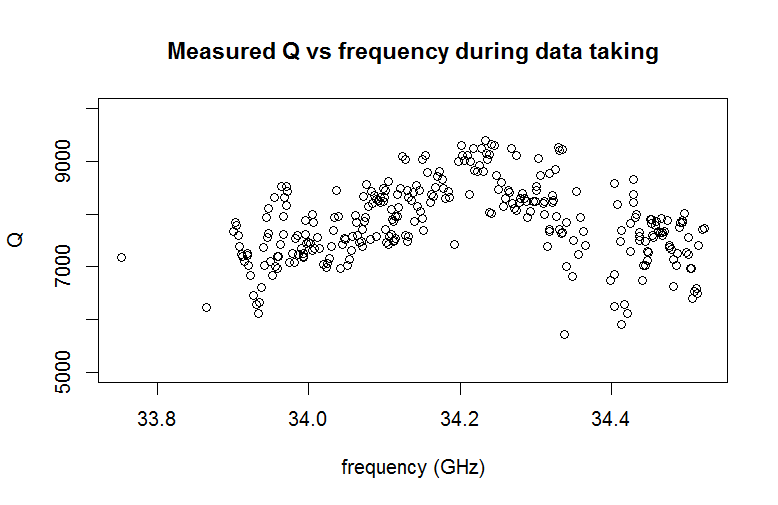
\includegraphics[width=1\textwidth]{measuredqvsfrequencyinsitucutoutoutlierswithtitle}
\end{figure}

Below is a plot of the form factor, calculated by simulating the electromagnetic fields in the cavity using the HFSS software.
\begin{figure}
\centering
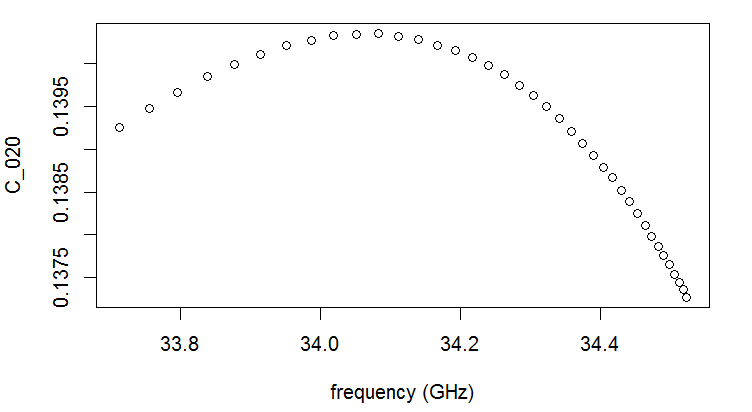
\includegraphics[width=1\textwidth]{formfactorvsfrequency}
\end{figure}

Shown below is a cross-sectional plot of the electric field in the z-direction for a dielectric rod with $\epsilon = 9.2$ inserted 0.028 inches into the cavity.

\begin{figure}
\centering
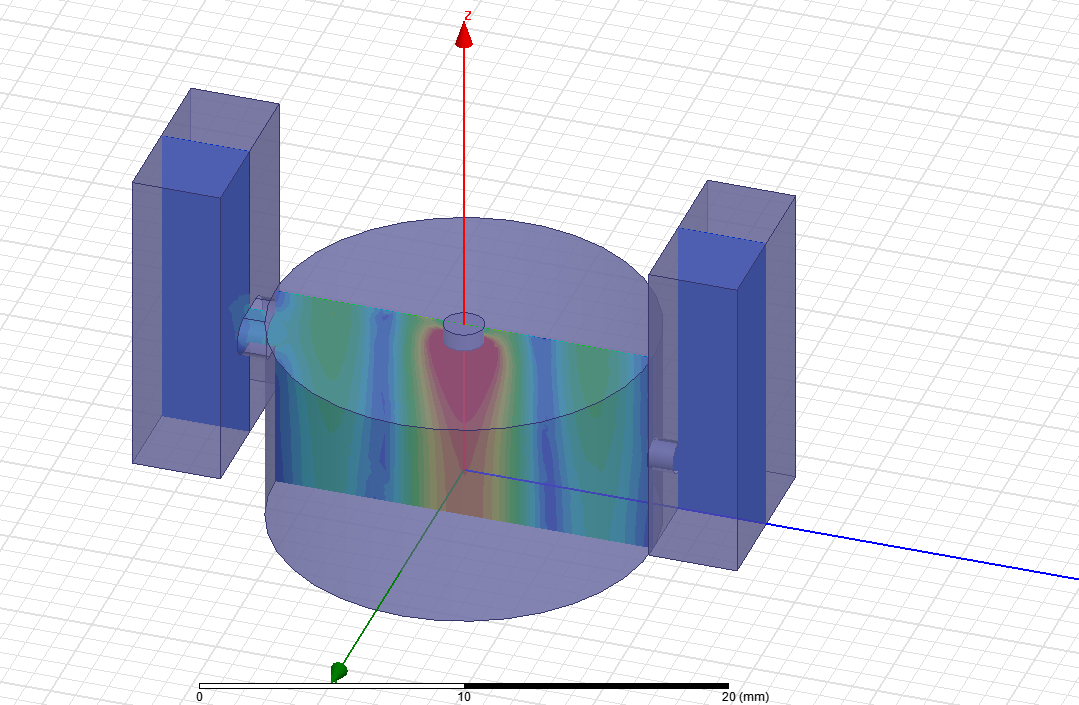
\includegraphics[width=0.8\textwidth]{efieldhfsssim28thou}
\end{figure}

Shown below is the frequency coverage NEED TO UPDATE

\begin{figure}
\centering
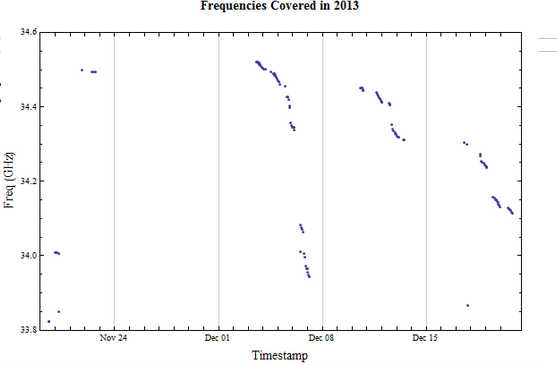
\includegraphics[scale=0.7]{frequencycoverage}
\end{figure}

\section{Data Analysis in Detail}
The data analysis starts from the raw time traces. The receiver chain at the final step separates the signal into an in-phase and quadrature component using an IQ mixer. These two separated signals each go through a low pass filter with approximately 4 MHz bandpass, and then are amplified by a voltage pre-amplifier with a gain of 5. The output channels (labeled henceforth as I and Q) are then plugged into a PCI 1154 card on a Dell desktop and digitized at a rate of 10 MSa/sec, with a a digital external referene at 10 MHz. We have a data acquisition program written in Visual C$\#$ that acquires however many records we desire, with each record containing 2.56e6 samples. The data acquisition has zero deadtime. The regular running procedure is to take 15,000 records at one particular cavity setting, and then retune - 15,000 records takes 1.06 hrs. 
Shown below is an example spectra

\begin{figure}
\centering
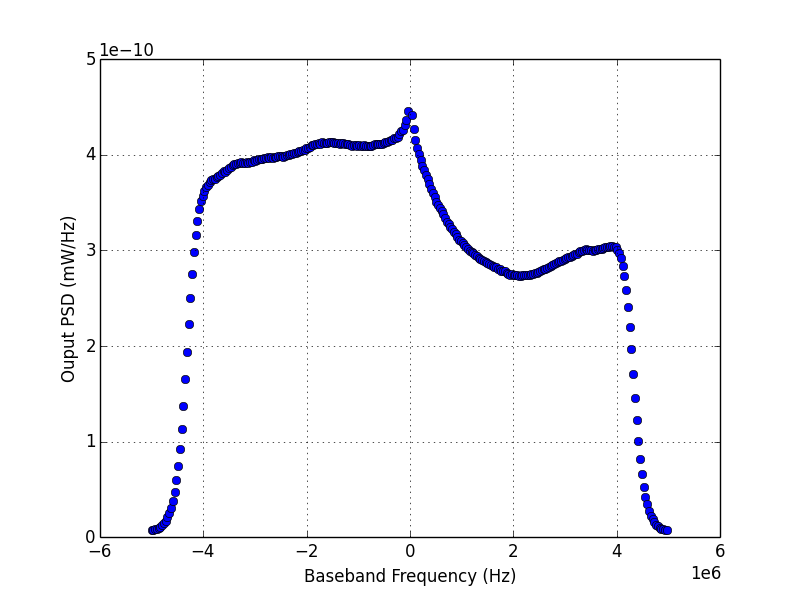
\includegraphics[width=\textwidth]{examplespectra}
\end{figure}

You can see the spike at 0 MHz which is our DC noise, the attenuation at the wings which is the result of the last 4 MHz Low-Pass filters, and the structure in the right hand side of the spectra, where the cavity is centered at 2 MHz. 

\subsection{cuts}

We discard all chunks that have the cavity drifting in frequency.

\begin{figure}
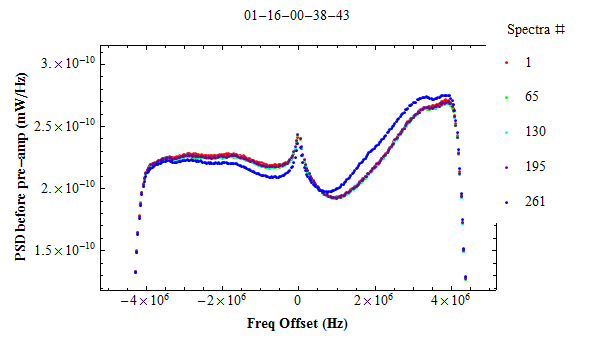
\includegraphics[width=\textwidth]{01-16-00-38-43}
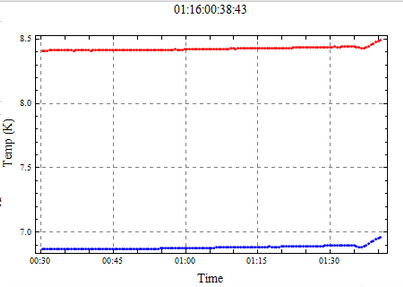
\includegraphics[width=\textwidth]{temp01-16-00-38-43}
\end{figure}
\begin{figure}
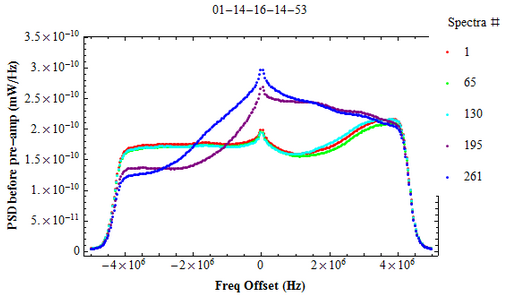
\includegraphics[width=\textwidth]{01-14-16-14-53}
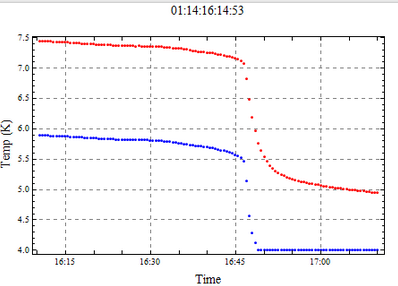
\includegraphics[width=\textwidth]{temp01-14-16-14-53}
\end{figure}

We also cut data when the temperature difference causes changes in the spectra.

\begin{figure}
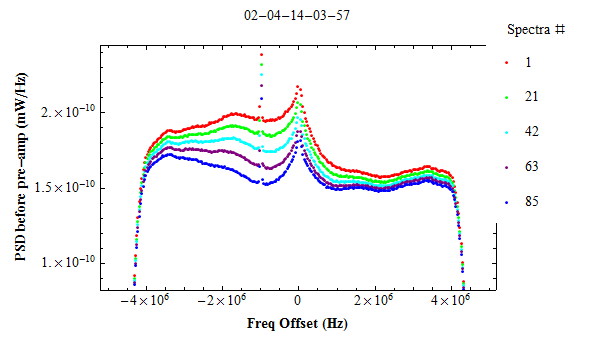
\includegraphics[width=\textwidth]{02-04-14-03-57}
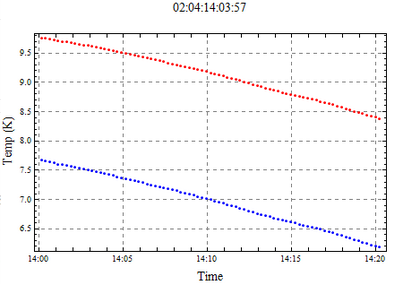
\includegraphics[width=\textwidth]{temp02-04-14-03-57}
\end{figure}
\begin{figure}
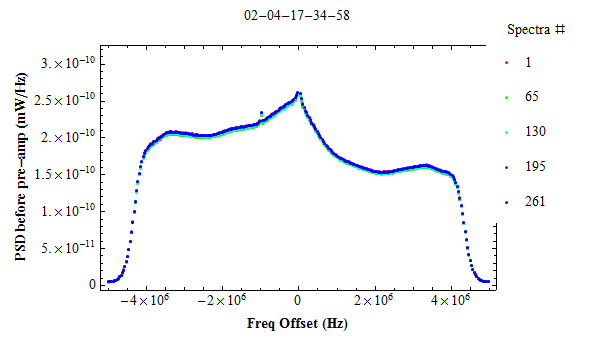
\includegraphics[width=\textwidth]{02-04-17-34-58}
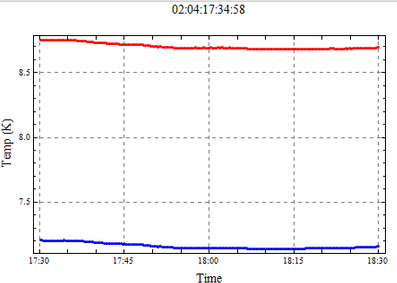
\includegraphics[width=\textwidth]{temp02-04-17-34-58}
\end{figure}

We take cuts on the data by removing the first 30 and last 30 points and also the 12 points in the middle where the DC spike occurs.

For runs taken after Jan 23, there was a test tone signal offset from the cavity resonance by -3 MHz to make sure we were seeing the correct structure. For these runs, the three bins centered on the test tone signal were cut as well. REALLY?

\centering 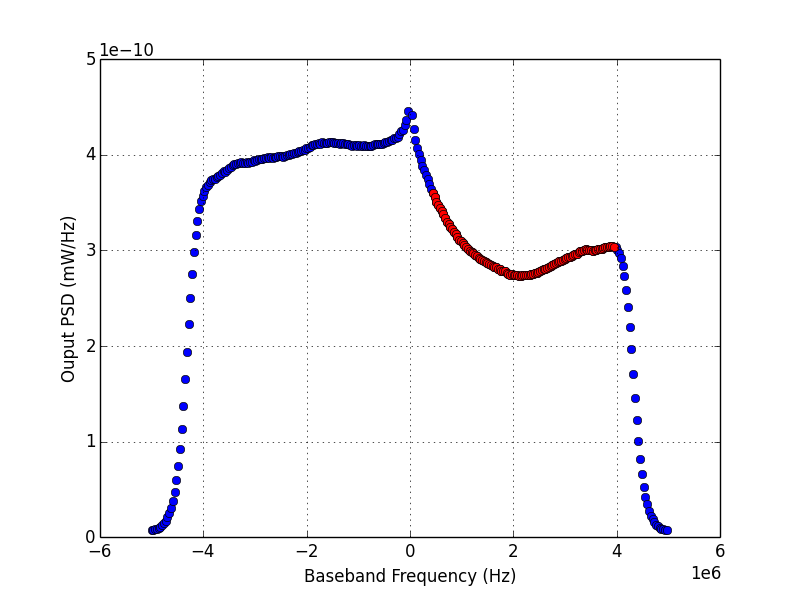
\includegraphics[width=0.6\textwidth]{cutondata}

We then do an empirical fit by smoothing the data using a moving average with window size of 3 bins. We subtract this smooth to get the fluctuations of the power spectrum about the local mean.

\begin{figure}
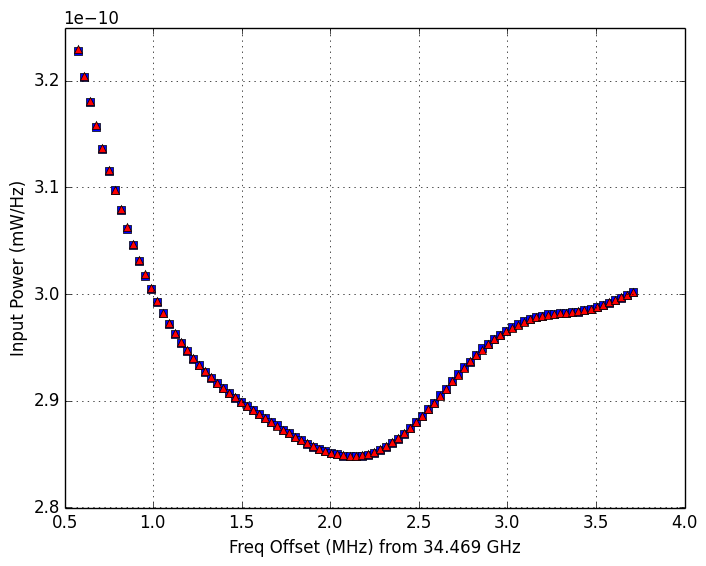
\includegraphics[width=0.8 \textwidth]{Dec04-11-33-24inputpltposfreq_237}
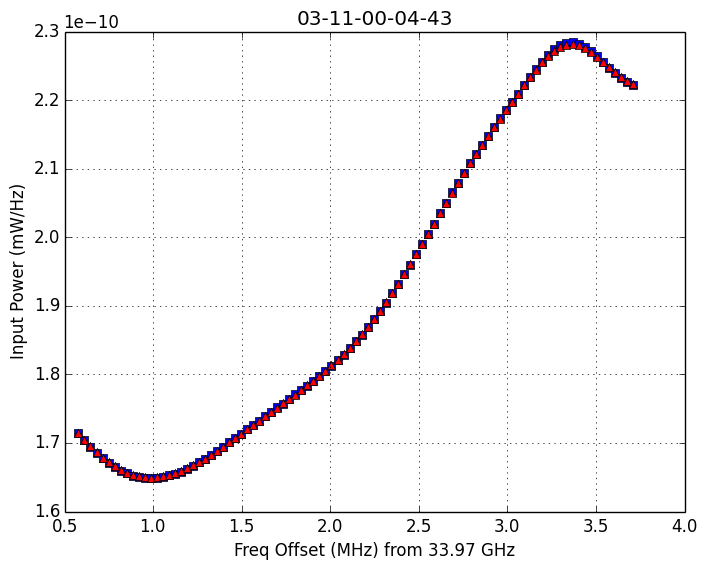
\includegraphics[width=0.8 \textwidth]{03-11-00-04-43inputpltposfreq_261}
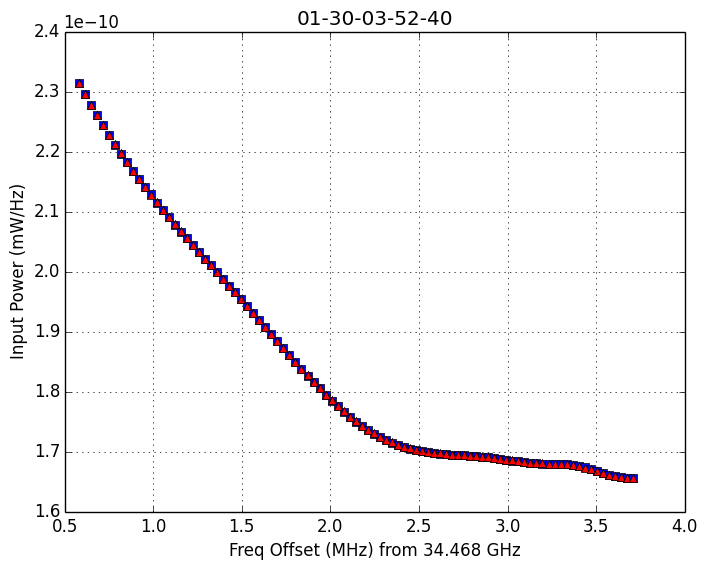
\includegraphics[width=0.8 \textwidth]{01-30-03-52-40inputpltposfreq_261}
\end{figure}

NEED TO UPDATE with figs with smooth (bin size  3). Here are the residuals of the subtraction for the above three timestamps: Point: shown here are the average of the residuals, where we discard spectra with significant temperature or frequency drifts. In the above timestamps, we were able to keep 90$\%$ of the data for the first timestamp, and all of the data for the second two.

\begin{figure}
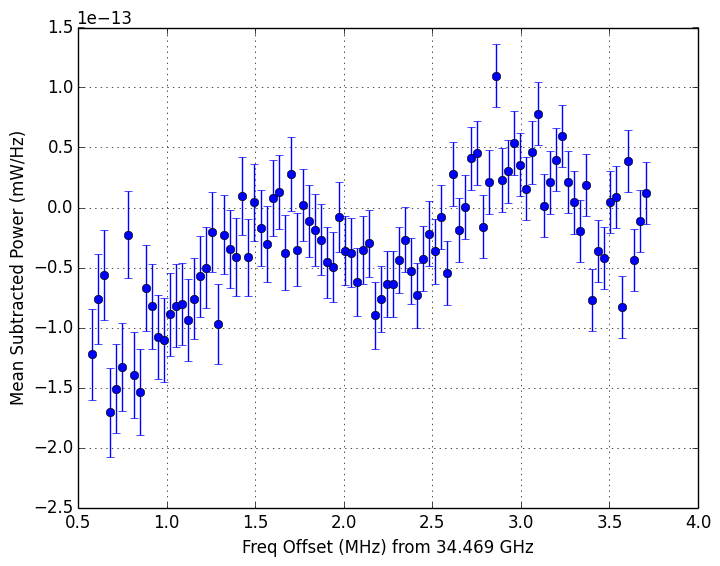
\includegraphics[width=0.8 \textwidth]{Dec04-11-33-24avgsubpltposfreq_237}
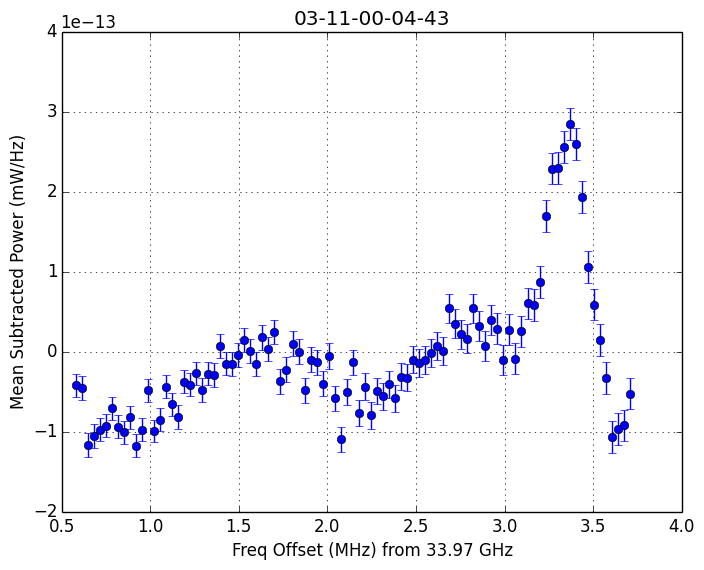
\includegraphics[width=0.8 \textwidth]{03-11-00-04-43avgsubpltposfreq_261}
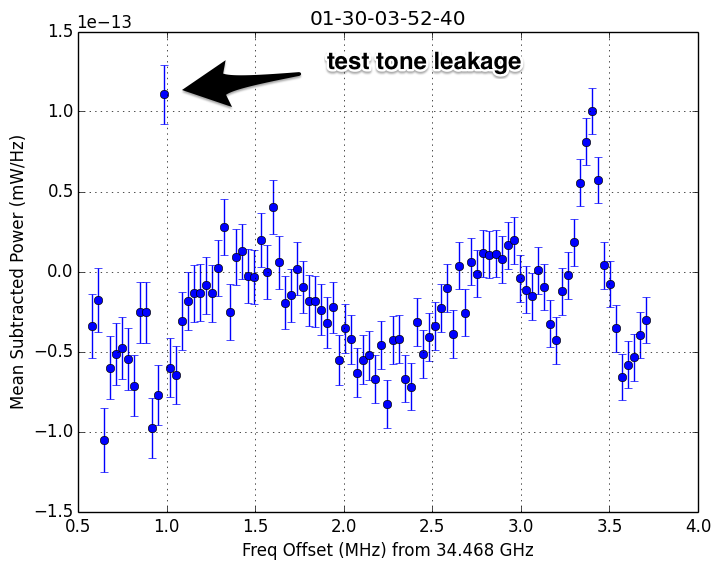
\includegraphics[width=0.8 \textwidth]{01-30-03-52-40avgsubpltposfreq_261}
\end{figure}


\end{document}